%======================================================================
\section{Introduction}
%======================================================================

Whether receiving help on an online platform motivates subsequent helping behavior has been a persistent question in the study of online communities. Generalized reciprocity, the tendency to help others after being helped oneself \citep{nowak_upstream_2007, baker_paying_2014}, is among the mechanisms proposed to sustain cooperation on platforms like Stack Overflow and Wikipedia, where direct exchange between the same two individuals is rare. If receiving help reliably increases the probability of giving it, cooperation may sustain itself through cascading helping acts, even among strangers \citep{fowler_cooperative_2010}. The behavioral evidence, however, is inconsistent: some observational studies find substantial reciprocity effects \citep{baker_paying_2014, chen_why_2019}, while others find weak or null relationships \citep{wasko_why_2005, joyce_predicting_2006}. We argue that much of this inconsistency is methodological.

Observational studies of reciprocity on platforms face a persistent confound: more engaged users are more likely both to seek help and to provide it, regardless of whether their own questions are resolved. Studies that correlate help received with help given, without accounting for this baseline activity, conflate reciprocity with general user engagement \citep{baker_paying_2014, chen_engaging_2018, joyce_predicting_2006}. A related limitation is that prior designs have largely treated receiving help as a one-time event, even though help-seeking and helping occur continuously.

We address both problems by developing a matched difference-in-differences survival analysis, applied to over 21 million questions from Stack Overflow. For each question a user posts, we define observation windows before and after the question and compare changes in helping behavior between users whose question received an answer (treated) and propensity-score-matched users whose question did not (control). We use Cox proportional hazards models to account for the continuous-time dynamics of helping behavior and the staggered, time-varying structure of treatment.

We develop two theoretical predictions alongside the basic reciprocity hypothesis. Drawing on theories of socialization and norm internalization, we predict that the reciprocity effect is stronger among newcomers than among experienced users (H2). Newcomers have not yet internalized community-specific norms or learned to value platform incentives such as reputation points; general moral obligations to reciprocate are therefore more likely to drive their behavior. As users accumulate experience, these general-purpose triggers may be displaced by community-specific motivations. We also predict that faster responses should amplify the reciprocity effect (H3), because gratitude is more intense when help arrives while the need is still salient \citep{mccullough_is_2001, tsang_gratitude_2006}.

The results support H1 and, with qualifications, H2, while offering only mixed support for H3. Relative to matched controls and to their own pre-question baseline, users who receive an answer help others at a modestly higher rate afterward (pooled HR\,$\approx$\,1.16), and this above-baseline elevation is largest among newcomers (HR\,$\approx$\,1.44 in the first week of tenure) and declines to near zero among the most experienced users (HR\,$\approx$\,1.04). One pattern complicates a purely reciprocal reading, and we foreground it rather than set it aside: much of the treated--control divergence emerges during the \textit{waiting period}, before the answer arrives --- a pre-trend we term \textit{anticipatory engagement} --- so the post-answer elevation partly reflects the heightened platform activity of users whose questions attract answers rather than a response to help received. We therefore report the treatment effect as the summed post- versus pre-question contrast, decompose it into its waiting-period and answer-arrival components, and treat the anticipatory-engagement pre-trend as an upper-bound qualification on the reciprocity interpretation throughout.

Our study makes three contributions. First, using a design built to remove the activity confound that inflates observational estimates, we provide field evidence that receiving help is associated with a modest increase in subsequent helping. Second, we show that this association is concentrated among newcomers and fades with experience, consistent with reciprocity functioning as a contributor-recruitment mechanism rather than a driver of sustained helping --- while also showing that much of the newcomer pattern is \textit{anticipatory engagement} that precedes the answer, which bounds how strongly the gradient can be read as reciprocity. Third, and methodologically, we show that entering the waiting period as an explicit term turns the parallel-trends assumption into a measured quantity, exposing a pre-answer divergence between treated and control users that a conventional before/after contrast would have absorbed into the treatment effect.

%======================================================================
\section{Theory}
%======================================================================

%----------------------------------------------------------------------
\subsection{Generalized Reciprocity}
%----------------------------------------------------------------------

A central mechanism proposed to support cooperation in online communities is \textit{generalized reciprocity}, the tendency for individuals who have received help to help others in turn, even when the recipient is not the original benefactor \citep{nowak_upstream_2007, fowler_cooperative_2010}. Unlike direct reciprocity, which involves returning favors to the same individual, generalized reciprocity requires no repeated interactions or exchange with the same person. Instead, it operates as a pay-it-forward model, sustaining collective contributions within groups where members may have infrequent or non-recurring interactions, such as online knowledge-sharing platforms.

Socio-psychological research identifies two complementary mechanisms underlying generalized reciprocity: moral reasoning and emotional responses. On the moral side, individuals may be guided by the logic of universalization \citep{levine_logic_2020}: they consider what would happen if all members requested more help than they gave. Such deliberation typically leads individuals to conclude that widespread free-riding would undermine the community as a valuable source of help, generating a shared moral obligation to reciprocate \citep{curry_is_2019}. This renders the relationship between individual and group into an indirect exchange: if one receives help from the group, one feels obligated to help the group in return.

Emotional mechanisms reinforce these moral considerations. A prominent response is gratitude, aroused by the perceived generosity of others \citep{mccullough_is_2001, mccullough_adaptation_2008}. Gratitude has been shown to motivate prosocial actions toward others beyond direct reciprocation \citep{tsang_gratitude_2006, bartlett_gratitude_2006}. According to \citet{molm_building_2007}, such emotional responses are especially relevant for systems where free riding is easy, such as online knowledge-sharing platforms. Experiencing gratitude in these contexts not only increases the propensity to help but also strengthens perceptions of the community as valuable and worth sustaining \citep{elster_norms_2009}.

Generalized reciprocity is among the most widely studied behavioral mechanisms explaining cooperative behavior in groups, owing to its potential to initiate cascading acts of generosity \citep{fowler_cooperative_2010, boyd_evolution_1989}. Comparative research and meta-analyses indicate that it is a globally shared moral principle \citep{curry_is_2019}. Robust experimental evidence comes from both laboratory \citep{greiner_indirect_2005, molm_building_2007, stanca_measuring_2009} and field settings \citep{mujcic_indirect_2018, fowler_cooperative_2010}.

%----------------------------------------------------------------------
\subsection{Empirical Challenges in Measuring Generalized Reciprocity}
%----------------------------------------------------------------------

Despite its theoretical importance, empirical findings on generalized reciprocity in online communities are mixed, and we argue that this inconsistency is largely attributable to persistent methodological challenges. Understanding these challenges is essential both for interpreting existing findings and for motivating our analytical approach.

A first challenge concerns the reliance on self-reported motives in surveys and interviews. Contributors frequently describe reciprocity as a central reason for their engagement \citep{wasko_it_2000, lakhani_how_2003}, yet sociological and psychological research has demonstrated that people have difficulty articulating the moral motives behind their actions \citep{vaisey_motivation_2009, mcclelland_how_1989}. When users state that they help because they enjoy it or feel a sense of obligation, it is unclear whether this reflects genuine reciprocity, altruism, conformity to perceived social norms, or the popular rhetoric of 'giving back' as a post-hoc rationalization. The distinction between reciprocity and other prosocial motives, such as the intrinsic joy of helping or the pursuit of social status, is particularly difficult for individuals to make through introspection \citep{batson1991altruism, benabou_incentives_2006}. As a result, self-reported data might overstate the prevalence of reciprocity as a discrete motive.

A second and more fundamental challenge is the endogeneity of help-seeking and help-giving in observational data. Users who ask questions on platforms like Stack Overflow are also disproportionately likely to answer questions, not because receiving help triggered a reciprocal response, but because both behaviors reflect the same underlying characteristics, such as greater platform engagement. Studies that correlate help received with help given without accounting for this baseline activity effectively confound reciprocity with user type \citep{baker_paying_2014, chen_engaging_2018, joyce_predicting_2006}. As we discuss below, the confound between reciprocity and user type is the central identification challenge that motivates our matched diff-in-diff design.

%----------------------------------------------------------------------
\subsection{Reciprocity and the User Trajectory}
%----------------------------------------------------------------------

We propose that the mixed findings in the literature can be partly reconciled by attending to a dimension that prior research has largely overlooked: the user trajectory from newcomer to experienced contributor. We argue that generalized reciprocity is strongest for new users and attenuates as users gain experience on the platform.

The logic of this prediction draws on theories of socialization and norm internalization. When a user first encounters an online community, they are unfamiliar with its specific norms, social structures, and reward systems. At this stage, community-specific incentives, such as reputation points, badges, or leaderboard positions, carry little motivational weight because the newcomer has not yet learned to value them. Instead, initial contributions are guided by more general moral principles that operate independently of community-specific knowledge. Generalized reciprocity is precisely such a principle: it requires only that the individual has received help and feels a moral obligation or emotional impulse to help in return, without any need to understand or identify with the particular community \citep{levine_logic_2020, curry_is_2019}.

As users interact with the community, they gradually learn its norms and develop a sense of membership. On platforms like Stack Overflow, these norms are codified in explicit reputation systems that reward helpful behavior with visible status markers. Once users internalize these community-specific norms, the broad moral obligation of reciprocity may be displaced by more localized incentive structures. The logic of universalization (``I should help because I was helped'') gives way to the logic of community membership (``I should help because that is what valued members do''). This norm displacement has been theorized in related contexts by \citet{benabou_incentives_2006}, who show how external incentives can crowd out moral motives.

Several additional mechanisms accelerate this decline. First, as users accumulate experiences of receiving help, each additional instance becomes less socially surprising and less likely to elicit strong gratitude \citep{mccullough_adaptation_2008}. The emotional response that fuels reciprocity habituates over time. Second, as users observe the platform's incentive structure that rewards helpful behavior with reputation and status, they may increasingly attribute others' helpful behavior to status pursuit rather than genuine generosity, further dampening the gratitude that triggers reciprocal helping.

This account predicts that generalized reciprocity is strongest among newcomers and declines with experience. This also helps explain why prior studies have reached different conclusions about the importance of reciprocity: those that focus on or oversample experienced users may underestimate reciprocity, while those that capture newcomer behavior may find stronger effects.

\hypmark{hyp:1}
\begin{quote}
\textsc{Hypothesis 1 (H1).} \emph{Receiving help increases a user's propensity to help others (generalized reciprocity effect).}
\end{quote}

\hypmark{hyp:2}
\begin{quote}
\textsc{Hypothesis 2 (H2).} \emph{The generalized reciprocity effect is strongest among newcomers and decreases as users gain experience on the platform.}
\end{quote}

%----------------------------------------------------------------------
\subsection{Response Time and the Immediacy of Reciprocity}
%----------------------------------------------------------------------

The emotional mechanisms underlying reciprocity suggest that the speed of help matters for the strength of reciprocity. Gratitude, the primary emotional driver of generalized reciprocity \citep{mccullough_is_2001}, is an affective response that is triggered by the perception of a benefactor's generosity. The intensity of this emotional response is likely to depend on the characteristics of the helping experience, including its timeliness.

A swift response to a help request can amplify the experience of receiving help through several channels. First, a fast answer signals that the community is attentive and generous, strengthening the perception that the group is worth sustaining through reciprocal contributions. Second, gratitude is an emotional response that may be most intense when it is temporally proximate to the perceived need. When a user posts a question, their need for help is salient; a quick answer arrives during this window of heightened need. The longer the user waits for help, the less valuable the help is and the more likely they are to have gotten help elsewhere. Thus, quick responses are likely to intensify feelings of gratitude.

Conversely, delayed responses may attenuate reciprocity. When an answer arrives hours or days after the question was posted, the user's original need may have faded; they may have found a solution elsewhere, or the problem may have become less pressing. The interval between asking and receiving weakens the associative link between the two events, potentially diluting the emotional response. Furthermore, longer waits may signal that the community is less responsive or generous, weakening the perception that underpins the moral obligation to reciprocate.

These considerations lead to a straightforward prediction:

\hypmark{hyp:3}
\begin{quote}
\textsc{Hypothesis 3 (H3).} \emph{Faster responses to a user's question strengthen the generalized reciprocity effect, while slower responses weaken it.}
\end{quote}

We note that this hypothesis follows from the dominant theoretical accounts of generalized reciprocity, which emphasize emotional immediacy and the salience of the helping experience. However, as we will show, field settings introduce structural dynamics, particularly the behavioral consequences of users being online and offline, that qualify the predictions of laboratory-based theory. We return to this issue when presenting our results.

%======================================================================
\section{Empirical Setting: Stack Overflow}
\label{sec:empirical_setting}
%======================================================================

Stack Overflow offers a valuable empirical setting for examining generalized reciprocity in online knowledge sharing. The platform provides publicly available quarterly data dumps containing rich longitudinal information on user behavior, including knowledge-seeking and knowledge-providing activities dating back to the platform's inception. This extensive dataset enables the reconstruction of helping patterns over time, allowing for the analysis of temporal sequences of receiving and providing help, which is critical for studying generalized reciprocity. We note that Stack Overflow activity has declined in recent years, partly due to the rise of generative AI tools; however, the core question-and-answer dynamics we study are shared broadly across help forums and knowledge-sharing communities, supporting the generalizability of the mechanisms we identify.

At its core, Stack Overflow is a question-and-answer platform for software developers and technologists. As of mid-2025, the site had accumulated over 24 million questions and 36 million answers from more than 4.5 million users. Its user base spans a wide range of experience levels and professional roles in software development and learners \citep{stack_overflow_stack_2024}. Questions on the platform must be tightly focused on specific programming problems; broad or opinion-based inquiries are typically closed by community moderation \citep{stack_exchange_inc_how_2024}. The most frequently discussed topics, as reflected in question tags, include JavaScript, Python, Java, C\#, PHP, Android, and HTML, spanning areas from web development and mobile applications to data science and machine learning. Stack Overflow is built around several core features: tags categorize questions by topic, facilitating expertise matching; a voting system allows users to upvote or downvote questions and answers to assess quality; and reputation points are earned for valued contributions such as providing high-quality answers; \citep{stack_exchange_inc_how_2024}.

For our study, the key feature is the question-and-answer interaction between users. When a user posts a question, other users may provide answers. This creates a clearly timestamped sequence (question posted, answer received) that we exploit to measure the temporal dynamics of generalized reciprocity. Crucially, on Stack Overflow, the identities of question-askers and answerers are typically different individuals, making this an ideal context for studying \textit{generalized} reciprocity: users who receive help from one community member may subsequently help entirely different members.

%======================================================================
\section{Data and Methods}
\label{sec:methods}
%======================================================================

To test our predictions, we develop a matched staggered difference-in-differences (DiD) survival analysis that leverages the temporal structure of help-seeking and help-giving on Stack Overflow. Our design compares changes in helping behavior (measured as the hazard of posting an answer) before and after an user receives an answer, between users who receive an answer and matched users who do not. This approach represents a novel integration of two methodological traditions: the staggered difference-in-differences framework of \citet{callaway_santanna_2021}, which accommodates variation in treatment timing and treatment effect heterogeneity, and the counting-process formulation of the Cox proportional hazards model \citep{andersen_gill_1982}, which allows treatment status and other covariates to vary continuously over the observation window.

%----------------------------------------------------------------------
\subsection{Study Design}
\label{sec:study_design}
%----------------------------------------------------------------------

For each question posted by a user, we construct a timeline centered on two key events: the posting of the question ($T_{\text{question}}$) and, for questions that receive an answer, the time at which the first answer with a non-negative vote score is posted ($T_{\text{answer}}$). We define an observation window spanning the two days before the question is posted ($T_{\text{question}} - 2\text{D}$) through the two days after ($T_{\text{question}} + 2\text{D}$). This yields a 4-day timeline for each question, divided into distinct phases.

We define three phases within each observation window (see Figure~\ref{fig:study_design}). The first phase, the \textit{pre-question phase}, is from the start of the observation window to the posting of the question ($T_{\text{question}} - 2\text{D}$ to $T_{\text{question}}$). This phase captures baseline helping activity before the focal question is asked.
The second phase, the \textit{waiting period} is from the posting of the question to the receipt of the first answer ($T_{\text{question}}$ to $T_{\text{answer}}$). During this interval, the user has asked for help but has not yet received it. 
The final \textit{post-answer phase} is from the receipt of the answer to the end of the observation window ($T_{\text{answer}}$ to $T_{\text{question}} + 2\text{D}$). This is the phase in which the reciprocity effect, if it exists, should manifest.

%% NEW (by SVPR)
A key feature of our design is that the post-answer (treated) phase begins at different elapsed times across observations, depending on how quickly the posted question receives a response.

This staggered timing of the post-answer phase corresponds to the setting studied by \citet{callaway_santanna_2021}, who show that standard two-way fixed-effects estimators can be biased when treatment timing varies, and treatment effects are heterogeneous. Our approach avoids this pitfall by explicitly modeling the time-varying change in treatment status within each observation window and by comparing treated observations only to not-yet-treated or never-treated controls.

For control users (those whose questions did not receive an answer), there is no natural transition between the waiting period and the post-answer phase. To maintain temporal alignment with the matched treated observation, we assign the control observation a synthetic phase transition at the same elapsed time as the treated user's response time. That is, if the treated user's answer was posted 4 hours after their question, the matched control observation's timeline is split at $T_{\text{question}} + 4\text{h}$, creating an aligned ``post'' phase of equal duration. This ensures that any differences between treated and control observations in the post-answer phase are not driven by differences in the length of the observation period.

The survival clock in our Cox models is centered on posting of the respective question: time zero corresponds to the start of the observation window ($T_{\text{question}} - 2\text{D}$), so that the question itself is posted at day~2 of the timeline and the observation window closes at day~4. All help events (answers posted by the focal user) are recorded with their exact timestamps and converted to elapsed time on this clock.

\begin{figure}
\caption{Study Design: Matched Difference-in-Differences Survival Analysis}
\label{fig:study_design}
\centering
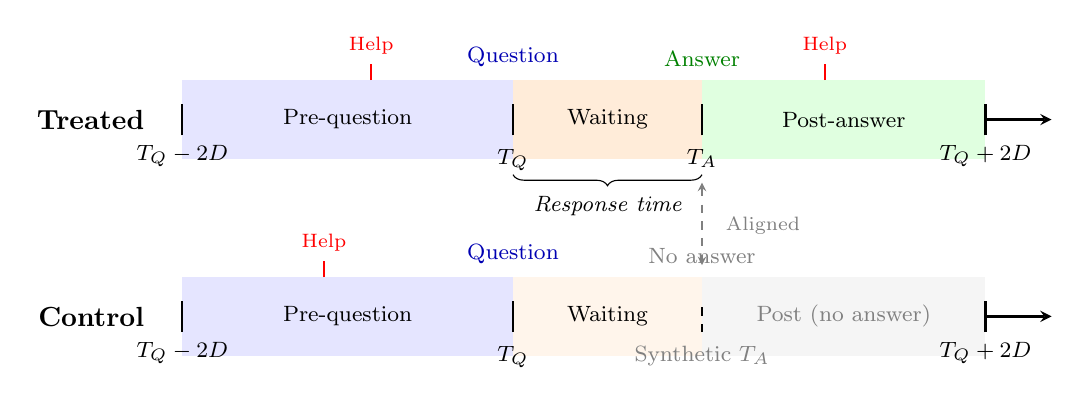
\begin{tikzpicture}[x=1.2cm, y=1cm, >=stealth, font=\small]
% --- Treated timeline ---
\node[anchor=east, font=\bfseries] at (-0.3, 2) {Treated};
% Main axis
\draw[thick, ->] (0,2) -- (9.2,2);
% Phase regions
\fill[blue!10] (0,1.5) rectangle (3.5,2.5);
\fill[orange!15] (3.5,1.5) rectangle (5.5,2.5);
\fill[green!12] (5.5,1.5) rectangle (8.5,2.5);
% Tick marks
\draw[thick] (0,1.8) -- (0,2.2);
\draw[thick] (3.5,1.8) -- (3.5,2.2);
\draw[thick] (5.5,1.8) -- (5.5,2.2);
\draw[thick] (8.5,1.8) -- (8.5,2.2);
% Labels below axis
\node[below, font=\footnotesize] at (0,1.8) {$T_Q - 2\text{D}$};
\node[below, font=\footnotesize] at (3.5,1.75) {$T_Q$};
\node[below, font=\footnotesize] at (5.5,1.75) {$T_A$};
\node[below, font=\footnotesize] at (8.5,1.8) {$T_Q + 2\text{D}$};
% Phase labels
\node[font=\footnotesize] at (1.75, 2) {Pre-question};
\node[font=\footnotesize] at (4.5, 2) {Waiting};
\node[font=\footnotesize] at (7.0, 2) {Post-answer};
% Response time brace
\draw[decorate, decoration={brace, amplitude=4pt, mirror}] (3.5, 1.3) -- (5.5, 1.3);
\node[below, font=\footnotesize\itshape] at (4.5, 1.15) {Response time};
% Question and answer markers
\node[above, font=\footnotesize, text=blue!70!black] at (3.5, 2.55) {Question};
\node[above, font=\footnotesize, text=green!50!black] at (5.5, 2.55) {Answer};
% --- Control timeline ---
\node[anchor=east, font=\bfseries] at (-0.3, -0.5) {Control};
% Main axis
\draw[thick, ->] (0,-0.5) -- (9.2,-0.5);
% Phase regions
\fill[blue!10] (0,-1) rectangle (3.5,0);
\fill[orange!8] (3.5,-1) rectangle (5.5,0);
\fill[gray!8] (5.5,-1) rectangle (8.5,0);
% Tick marks
\draw[thick] (0,-0.7) -- (0,-0.3);
\draw[thick] (3.5,-0.7) -- (3.5,-0.3);
\draw[thick, dashed] (5.5,-0.7) -- (5.5,-0.3);
\draw[thick] (8.5,-0.7) -- (8.5,-0.3);
% Labels below axis
\node[below, font=\footnotesize] at (0,-0.7) {$T_Q - 2\text{D}$};
\node[below, font=\footnotesize] at (3.5,-0.75) {$T_Q$};
\node[below, font=\footnotesize, text=gray] at (5.5,-0.75) {Synthetic $T_A$};
\node[below, font=\footnotesize] at (8.5,-0.7) {$T_Q + 2\text{D}$};
% Phase labels
\node[font=\footnotesize] at (1.75, -0.5) {Pre-question};
\node[font=\footnotesize] at (4.5, -0.5) {Waiting};
\node[font=\footnotesize, text=gray] at (7.0, -0.5) {Post (no answer)};
% Question marker
\node[above, font=\footnotesize, text=blue!70!black] at (3.5, 0.05) {Question};
\node[above, font=\footnotesize, text=gray] at (5.5, 0.05) {No answer};
% Alignment arrows
\draw[dashed, gray, <->] (5.5, 1.2) -- (5.5, 0.15);
\node[right, font=\scriptsize, text=gray] at (5.65, 0.65) {Aligned};
% Help events (example)
\draw[red, thick] (2.0, 2.5) -- (2.0, 2.7) node[above, font=\scriptsize, text=red] {Help};
\draw[red, thick] (6.8, 2.5) -- (6.8, 2.7) node[above, font=\scriptsize, text=red] {Help};
\draw[red, thick] (1.5, 0) -- (1.5, 0.2) node[above, font=\scriptsize, text=red] {Help};
\end{tikzpicture}

\vspace{0.5em}
\parbox{\textwidth}{\footnotesize\textit{Note.} Each observation window spans 4 days centered on the focal question ($T_Q$). The treated timeline (top) shows three phases: the pre-question phase (baseline), the waiting period (question posted, no answer yet), and the post-answer phase (after the first qualifying answer $T_A$ arrives). The control timeline (bottom) is from a propensity-score-matched user whose question did not receive an answer. To ensure temporal alignment, the control's post-question period is split at a synthetic transition point matching the treated user's response time. Red markers indicate help events (answers posted by the focal user to other users' questions). The treatment effect is the differential change in helping hazard between treated and control observations in the post-answer phase, relative to the pre-question baseline. The staggered timing of $T_A$ across observations motivates our use of matched DiD.}
\end{figure}

Within each timeline, we track all instances in which the user provides an answer to another user's question. These helping events constitute the outcome in our survival analysis. Conceptually, our design asks: Does the hazard of helping increase after a user receives an answer, relative to the change in hazard for a matched user who does not receive an answer? We present descriptive evidence on the raw help rates over this timeline in Section~\ref{sec:results} (Figure~\ref{fig:help_rate_pooled}), before turning to the formal Cox model estimates.

%----------------------------------------------------------------------
\subsection{Data}
%----------------------------------------------------------------------

We utilized the full sample of non-deleted questions from Stack Overflow's inception on 31 July 2008 through 1 April 2025. We addressed two edge cases that would render our fixed-length observation window invalid. First, for early platform questions, the pre-period could predate the platform's launch, meaning no answers were possible at that time. We removed 1,080 such cases. Second, due to the data dump's April~1, 2025, cut-off, the post-period could be prematurely truncated. We excluded 8,029 cases affected by this. We then excluded 2,671,121 questions that received an answer from the question poster. These filtering steps resulted in a pre-matching dataset of 21,033,429 questions from 4,764,048 unique users. After propensity score matching (described below), the matched file comprises 24,527,534 question-level rows (12,263,767 matched pairs; some control questions appear more than once) from 3,899,114 unique users, with a 50\% treatment rate by construction. The Cox analytic sample retains 16,252,524 unique questions with non-missing response-time alignment.

%----------------------------------------------------------------------
\subsection{Variables}
%----------------------------------------------------------------------

Table~\ref{tab:variables} provides an overview of the variables used in our analysis. The phase terminology is consistent with Figure~\ref{fig:study_design}: the pre-question phase captures baseline behavior, the waiting period spans the interval from question to answer, and the post-answer phase captures the period after the answer arrives. We use ``post-question'' to refer to the combined waiting period and post-answer phase whenever distinguishing between these two sub-periods is not necessary.

\begin{table}
\caption{Overview of Variables}
\label{tab:variables}
\centering
\begin{tabularx}{\textwidth}{@{}lX@{}}
\toprule
\textbf{Variable} & \textbf{Description} \\
\midrule
\multicolumn{2}{@{}l}{\textit{Outcome (Survival Event)}} \\
\hspace{1em} helpEvent & A binary event indicator equal to 1 at times when the user posts an answer to another user's question within the observation window. \\
\midrule
\multicolumn{2}{@{}l}{\textit{Time-Varying Covariates}} \\
\hspace{1em} PostQuestion & Binary; 1 for intervals occurring after the user posts their question ($t \geq T_{\text{question}}$), 0 otherwise. Captures the combined post-question period (waiting period + post-answer phase). \\
\hspace{1em} PostAnswer & Binary; 1 for intervals occurring after the user receives their first answer ($t \geq T_{\text{answer}}$), 0 otherwise. For control users (no answer received), this variable switches on at the synthetic transition point at the matched treated user's response time. Isolates the post-answer phase. \\
\hspace{1em} treatedPostQuestion & Interaction of treatment $\times$ phasePostQuestion; captures differential behavior of treated users in the entire period after the question. \\
\hspace{1em} isTreatedActive & Interaction of treatment $\times$ phasePostAnswer; the primary treatment effect capturing the additional lift in helping hazard after receiving an answer, beyond any change attributable to the act of asking a question. \\
\hspace{1em} ResponseTime & Time between question and the first answer (excluding down-voted answers) of the treated question. We include interactions with all four variables above. \\
\bottomrule
\end{tabularx}
\end{table}

\paragraph{Outcome.} The event of interest in our survival analysis is the posting of an answer. Within each observation window, we track when (and whether) the focal user provides an answer to any other user's question. The Cox model estimates the instantaneous hazard of this helping event as a function of time-varying covariates that capture the phase of the observation timeline and the treatment status.

\paragraph{Treatment.} The treatment is the receipt of an answer. We operationalize this using \textit{treatment}, a binary variable indicating whether the user's question received at least one answer with a non-negative score. We adopt this operationalization rather than Stack Overflow's ``accepted answer'' mechanism to address endogeneity: marking an answer as accepted requires the user to return to the site, which may itself correlate with helping behavior.

\paragraph{Response Time.} For each treated observation, the response time variable used in the interaction terms is $\log(1 + t_{\text{answer}})$, where $t_{\text{answer}}$ is the elapsed time in hours from the start of the observation window ($T_Q - 2\text{D}$) to the arrival of the first answer with a non-negative vote score. Because $T_Q - 2\text{D}$ is a fixed origin common to all observations, this is a monotone transformation of the actual response time in hours ($t_{\text{answer}} - t_{\text{question}}$) and preserves the full ordering of fast versus slow answers; however, it shifts the scale by the constant pre-question window length. For numerical stability, both response-time interaction terms ($\text{isTreatedActive} \times \log(1+t_{\text{answer}})$ and $\text{treatedPostQuestion} \times \log(1+t_{\text{answer}})$) are clipped to their 5th--95th percentile range and then standardized (z-scored) before model fitting. Consequently, the reported interaction coefficients $\gamma$ and $\delta$ are expressed per one standard deviation of the respective interaction term rather than per unit of $\log(1+t_{\text{answer}})$.

\paragraph{User Experience.} To test Hypothesis 2, we stratify our analysis by user tenure, defined as the number of days between a user's first activity on the platform and the start of the observation window. We define seven tenure buckets using right-closed intervals: $[0, 7]$, $(7, 30]$, $(30, 180]$, $(180, 365]$, $(365, 1095]$, $(1095, 2190]$, and $(2190, \infty)$ days, corresponding to the labels less than one week, one week to one month, one to six months, six to twelve months, one to three years, three to six years, and more than six years, respectively. Running separate models by bucket enables us to examine how the reciprocity effect varies across the user trajectory without imposing a parametric functional form. 

%----------------------------------------------------------------------
\subsection{Propensity Score Matching}
\label{sec:matching}
%----------------------------------------------------------------------

Because the receipt of an answer (the treatment) is correlated with user characteristics (more experienced users, for instance, might tend to ask higher-quality questions that are more likely to receive answers), we employ propensity score matching \citep{rosenbaum_rubin_1983} to improve the comparability of the treatment and control groups. Importantly, matching is performed \textit{across different users}: each treated question (from a user who received an answer) is matched to a control question (from a different user whose question did not receive an answer) that has a similar propensity to receive an answer based on observable pre-treatment characteristics. This cross-user matching ensures that treated and control observations are independent conditional on the matched covariates, while the DiD structure within each pair absorbs residual differences.

We estimate the propensity score using the following pre-treatment covariates, which jointly capture user experience, recent activity, and question characteristics as depicted in Table \ref{tab:covariates}. It should be noted that \textit{tagAnswerRateAvg} is critical for addressing the concern that question complexity may confound the treatment: questions in tags with low answer rates are inherently more difficult, and matching on this rate ensures that treated and control questions come from similarly tractable topic areas.
Matching on the tag-level answer rate is particularly important for our response time analysis, as it mitigates the concern that slower response times simply proxy for differently sized sub-communities with lower throughput. We use nearest-neighbor matching with a caliper of 0.05 on the propensity score.

\begin{table}
\caption{Definition of Matching Covariates}
\label{tab:covariates}
\centering\small
\begin{tabular}{p{4cm} p{9cm}}
\toprule
\textbf{Variable name} & \textbf{Definition} \\
\midrule
\textit{Exact matching} & \\
calendarYear & Calendar year exact matching indicating the year of the observation, controlling for secular trends in platform activity and answer rates. \\
topLevelTag & First tag of the question indicating the main topic and community that sees the question \\

\multicolumn{2}{l}{\textit{Propensity score matching}}\\
userTenure & Number of days since the user's first recorded activity on the platform, capturing cumulative experience. \\
numQuestionsAskedAT & Total number of questions asked by the user prior to the observation window. \\

numHelpProvidedAT & Total number of answers provided by the user prior to the observation window. \\

numQuestionsAsked30D & Number of questions asked in the 30 days preceding the observation window. \\

numHelpProvided30D & Number of answers provided in the 30 days preceding the observation window. \\

numQuestionsAsked7D & Number of questions asked in the 7 days preceding the observation window. \\

numHelpProvided7D & Number of answers provided in the 7 days preceding the observation window. \\

tagAnswerRateAvg & Average share of questions that receive an answer within the question's tags, capturing topic-specific difficulty. \\
\bottomrule
\end{tabular}
\end{table}

\iffalse
\begin{itemize}
    \item \textit{User tenure}: the number of days since the user's first activity on the platform, capturing cumulative experience.
    \item \textit{Cumulative activity}: total questions asked and total answers provided before the observation window.
    \item \textit{Recent activity}: questions asked and answers provided in the 30 days and 7 days before the observation window, capturing current engagement intensity.
    \item \textit{Pre-question helping}: whether the user provided any help during the pre-question phase, capturing baseline helping propensity.
    \item \textit{Tag-level answer rate}: the average share of questions that receive an answer within the question's tags, capturing topic-specific difficulty and demand. This variable is critical for addressing the concern that question complexity may confound the treatment: questions in tags with low answer rates are inherently more difficult, and matching on this rate ensures that treated and control questions come from similarly tractable topic areas.
    \item \textit{Calendar year}: to account for secular trends in platform activity and answer rates.
\end{itemize}
\fi

Table~\ref{tab:balance} displays the covariate balance before and after matching. Before matching, several covariates showed a meaningful imbalance between the treated and control groups. For instance, treated users had asked more questions in the prior 30 days (SMD\,=\,0.197) and 7 days (SMD\,=\,0.174), reflecting that users who ask questions that attract answers tend to be more recently active. The largest imbalance was in the tag-level answer rate (SMD\,=\,0.695), confirming that question topic characteristics strongly predict answer receipt and underscoring the importance of matching on this variable. After nearest-neighbor propensity score matching, all standardized mean differences fell well below the conventional threshold of 0.1, with the largest residual imbalance at 0.029 (see Table~\ref{tab:balance}). This confirms adequate balance across all matching covariates, and the balance is also illustrated in the Love plot in Appendix~\ref{sec:balance_plot}.

\begin{table}
\caption{Covariate Balance Before and After Matching}
\label{tab:balance}
\centering\small
\adjustbox{max width=\textwidth}{%
\begin{tabular}{lcccccc}\toprule
 & \multicolumn{3}{c}{Unmatched} & \multicolumn{3}{c}{Matched} \\ \cmidrule(lr){2-4} \cmidrule(lr){5-7}
 Covariate & Tr Mean & Ct Mean & SMD & Tr Mean & Ct Mean & SMD \\\midrule
 userTenure & 570.95 & 720.62 & $-$0.167 & 569.58 & 568.20 & 0.002 \\
 numQuestionsAskedAT & 31.11 & 26.00 & 0.059 & 30.75 & 30.19 & 0.006 \\
 numHelpProvidedAT & 15.27 & 14.15 & 0.009 & 14.70 & 12.87 & 0.018 \\
 numQuestionsAsked30D & 2.00 & 1.19 & 0.197 & 1.98 & 1.96 & 0.004 \\
 numHelpProvided30D & 0.81 & 0.46 & 0.068 & 0.78 & 0.63 & 0.029 \\
 numQuestionsAsked7D & 0.57 & 0.34 & 0.174 & 0.56 & 0.56 & $-$0.001 \\
 numHelpProvided7D & 0.22 & 0.12 & 0.063 & 0.21 & 0.17 & 0.028 \\
 tagAnswerRateAvg & 0.51 & 0.44 & 0.695 & 0.51 & 0.51 & 0.004 \\
\bottomrule\end{tabular}}%

\vspace{0.3em}
\parbox{0.9\textwidth}{\footnotesize\textit{Note.} SMD = standardized mean difference. The conventional threshold for acceptable balance is $|\text{SMD}| < 0.1$. All post-matching SMDs fall well below this threshold.}
\end{table}

%----------------------------------------------------------------------
\subsection{Analytical Strategy: Cox Proportional Hazards with Time-Varying Covariates}
%----------------------------------------------------------------------

We model the hazard of helping using a Cox proportional hazards model with time-varying covariates \citep{andersen_gill_1982}. The counting-process formulation of \citet{andersen_gill_1982} extends the original Cox model (\citep{cox_regression_1972} to settings with time-varying covariates and recurrent events, providing the large-sample theoretical foundation (including consistency and asymptotic normality of the partial likelihood estimator) that justifies our approach.

For each matched pair of observations (one treated, one control), we partition the 4-day observation window into intervals defined by the key event times: the start of the window, the posting of the question, and the arrival of the answer (the actual answer arrival for treated users or the synthetic transition for controls).

The hazard function is specified as:

\begin{multline}
\label{eq:cox}
h(t \mid \mathbf{X}(t)) = h_0(t) \exp\big(\beta_0 \cdot \text{treatment} + \beta_1 \cdot \text{phasePostQuestion}(t) + \beta_2 \cdot \text{treatedPostQuestion}(t) \\
+ \beta_3 \cdot \text{phasePostAnswer}(t) + \beta_4 \cdot \text{isTreatedActive}(t) \big)
\end{multline}

\noindent where $h_0(t)$ is the baseline hazard. \textit{treatment} is a time-constant indicator for treatment group membership (1 if the user's question received an answer, 0 otherwise); it absorbs stable between-group differences in baseline helping rates. The remaining covariates are time-varying indicators that switch on at the appropriate event times. Because \textit{treatedPostQuestion} switches on when the question is posted and remains on through the post-answer phase, the post-answer treatment effect is not the \textit{isTreatedActive} coefficient in isolation but the sum $\beta_2 + \beta_4$ --- the difference, between treated and control users, in the change in helping hazard from the pre-question baseline to the post-answer phase. We report this summed difference-in-differences contrast as the treatment effect, together with its two components: $\beta_2$, the waiting-period divergence, and $\beta_4$, the increment at answer arrival net of that divergence.

To test the moderation by response time (Hypothesis 3), we extend the model with two additional terms:

\begin{multline}
\label{eq:cox_speed}
h(t \mid \mathbf{X}(t)) = h_0(t) \exp\Big(\boldsymbol{\beta}' \mathbf{X}(t) \\
+ \gamma \cdot \text{isTreatedActive}(t) \times \widetilde{\log}(\text{RT}) + \delta \cdot \text{treatedPostQuestion}(t) \times \widetilde{\log}(\text{RT}) \Big)
\end{multline}

\noindent where $\widetilde{\log}(\text{RT})$ denotes the standardized log response-time variable (see below), $\gamma$ captures the moderation of the answer-arrival increment by answer speed, and $\delta$ captures the analogous moderation during the waiting period. Just as the base treatment effect is the sum $\beta_2 + \beta_4$, the response-time moderation of that effect is the sum $\gamma + \delta$; we report this net moderation alongside its two components. A negative $\gamma + \delta$ would indicate that faster answers strengthen the reciprocity effect (consistent with H3), while a positive sum would indicate the opposite.

\paragraph{Stratification by Tenure.} To test Hypothesis 2, we fit separate models for each of the seven tenure buckets. This allows the baseline hazard and all coefficients to vary freely across levels of user experience, providing a nonparametric view of how reciprocity changes over the user trajectory.

\paragraph{Identification.} Our identification strategy rests on the matched DiD logic embedded in the model. Propensity score matching \citep{rosenbaum_rubin_1983} ensures that treated and control observations come from users with comparable baseline characteristics, including tenure, activity levels, and question topic difficulty. This matching absorbs between-user differences that might otherwise confound the treatment effect. We do not include user fixed effects in the survival models. Because matching is performed across different users (not within-user), and because the Cox model already leverages within-observation temporal variation through the time-varying covariate structure \citep{andersen_gill_1982}, user fixed effects are not required for identification. The DiD structure compares within-observation changes before and after the answer across treatment groups, isolating the treatment effect from stable individual differences. The waiting-period covariate (\textit{treatedPostQuestion}) captures any lift in helping that treated users show after asking but before receiving an answer. When this term is near zero, treated and control users move in parallel up to the answer, and the summed post-answer effect can be read as the effect of answer receipt; when it is large, the two groups diverge before treatment arrives, and the summed effect blends this pre-answer divergence with any response to the answer itself. We therefore report the waiting-period term explicitly, so that departures from parallel trends are measured rather than assumed away, and we return to its magnitude in the Results.

%======================================================================
\section{Results}
\label{sec:results}
%======================================================================

%----------------------------------------------------------------------
\subsection{Descriptive Statistics}
%----------------------------------------------------------------------

The Cox analytic sample spans 16,252,524 question-level observations from 3,899,114 unique users on Stack Overflow, with 50\% of questions receiving at least one answer. Help-event counts are right-skewed: the mean is 0.65 events per observation window (SD\,=\,2.33), consistent with helping being a relatively rare behavior for any individual user in any given window. Among treated users, the median response time from question to first answer is 0.34 hours, though the distribution is heavily right-skewed (mean 5.09 hours, SD\,=\,17.09), reflecting a minority of questions that wait many hours or days for a response. The sample spans all levels of platform experience, with the largest strata being established users (1--3 years: $n=4{,}312{,}164$) and newcomers ($<$\,1 week: $n=2{,}667{,}533$).

\begin{table}[H]
\caption{Descriptive Statistics}
\label{tab:desc_stats}
\centering
\begin{tabular}{@{}lrrrr@{}}
\toprule
\textbf{Variable} & \textbf{Mean} & \textbf{SD} & \textbf{Median} & \textbf{N} \\
\midrule
Questions (observations) & & & & 4,804,183 \\
Unique users & & & & 908,775 \\
\% questions with answer & 50.00\% & & & \\
\midrule
Help events per window & 0.85 & 8.25 & 0.00 & \\
User tenure (days) & 706 & 788 & 434 & \\
Response time (hours, treated) & 5.78 & 18.76 & 0.33 & \\
\midrule
\multicolumn{5}{@{}l}{\textit{Observations by Tenure Bucket}} \\
\hspace{1em} < 1 Week & & & & 153,253 \\
\hspace{1em} 1 Week - 1 Month & & & & 281,257 \\
\hspace{1em} 1 - 6 Months & & & & 951,558 \\
\hspace{1em} 6 - 12 Months & & & & 765,542 \\
\hspace{1em} 1 - 3 Years & & & & 1,614,190 \\
\hspace{1em} 3 - 6 Years & & & & 740,459 \\
\hspace{1em} > 6 Years & & & & 297,924 \\
\bottomrule
\end{tabular}
\end{table}


%----------------------------------------------------------------------
\subsection{Descriptive Evidence: Help Rates and the Parallel Trends Assumption}
%----------------------------------------------------------------------

\begin{figure}[h]
\centering
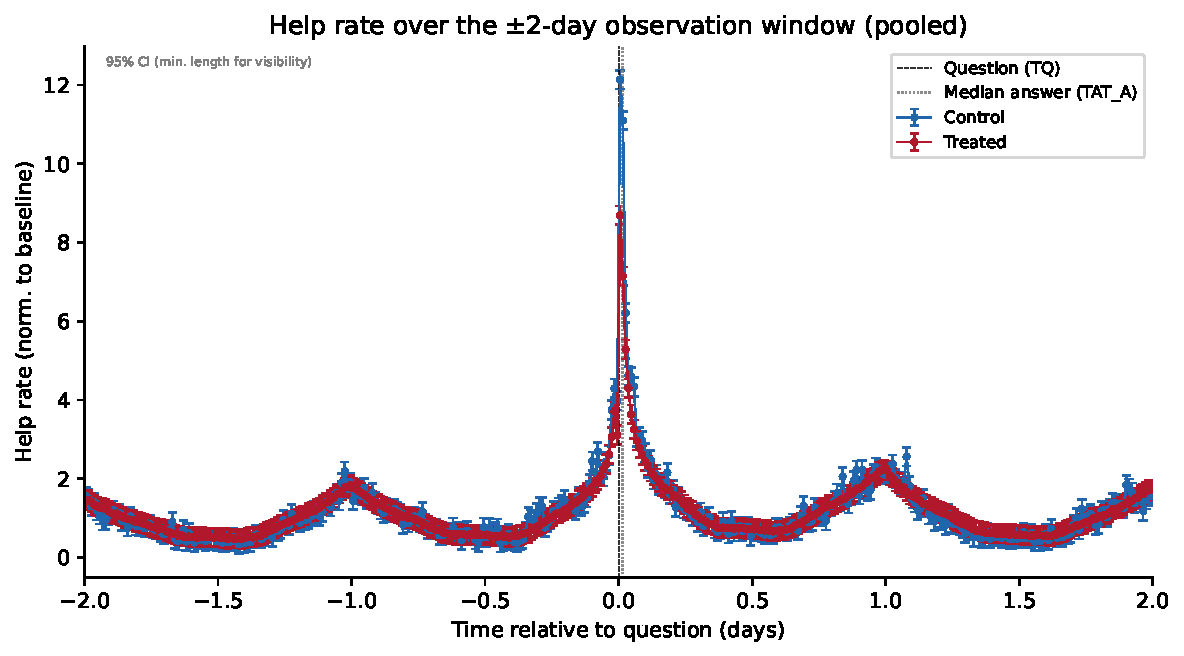
\includegraphics[width=\textwidth]{analysis/output_figures/help_rate_pooled.pdf}
\caption{Help rate over the $\pm$4-day observation window, pooled across all tenure buckets. The normalized help rate (relative to each group's pre-question baseline) is plotted for treated users (red, who received an answer) and matched control users (blue, who did not).}
\label{fig:help_rate_pooled}
\end{figure}

Figure~\ref{fig:help_rate_pooled} plots the normalized help rate for treated and control users over the two days before and after question posting. Before the question ($t < T_Q$), treated and control help rates track each other closely, consistent with the parallel-trends assumption and with the effectiveness of propensity-score matching: the two groups enter the window with comparable baseline helping propensities. The groups begin to diverge \textit{after} the question is posted but \textit{before} the median answer arrives, and treated users' help rate remains above that of controls through the post-answer phase. This waiting-period divergence --- anticipatory engagement --- is the descriptive counterpart of the large waiting-period coefficient reported below, and it cautions against attributing the full post-answer gap to the arrival of the answer. % TODO(re-run): regenerate help_rate_pooled from the revision event histories (help_rate_over_time.py) and confirm the pre-question overlap and the waiting-period divergence in the refreshed figure.

%----------------------------------------------------------------------
\subsection{Generalized Reciprocity Effect (H1)}
%----------------------------------------------------------------------


% =====================================================================
% NUMERICS: point estimates below are from the current (with-accepts) run and
% are exact from the committed coefficients. After the clean re-run (accept
% events excluded; see create_matched_event_histories.py), refresh every HR/CI
% from the regenerated \input tables. The qualitative structure is robust:
% positive but modest summed effect, a large waiting-period (anticipatory-
% engagement) term, a negative answer-arrival increment, and a tenure gradient
% carried mainly by the waiting-period term.
% AUTHOR DECISION: how hard to foreground the anticipatory-engagement pre-trend
% versus the positive summed effect is a framing call — flagged at each turn below.
% =====================================================================
To test Hypothesis~1, we estimate the pooled Cox model across all experience levels (Table~\ref{tab:pooled_experienced}). The treatment effect --- the summed post- versus pre-question contrast ($\beta_2 + \beta_4$) --- is positive: relative to matched controls and to their own pre-question baseline, treated users help others at an approximately 16\% higher hazard once their question has been answered (HR\,$\approx$\,1.16, $p < .001$). This is consistent with generalized reciprocity, and its magnitude is modest, in line with the view that designs which do not net out baseline activity overstate the effect.

The decomposition, however, complicates a purely reciprocal reading. Almost all of the treated--control divergence opens during the waiting period, before any answer arrives: the waiting-period coefficient is large and positive (\textit{Received Answer $\times$ Post-Question}, coefficient\,$\approx$\,1.39, $p < .001$), whereas the increment at answer arrival is itself negative (\textit{isTreatedActive}, coefficient\,$\approx\,-1.24$, $p < .001$). We label this pre-answer divergence \textit{anticipatory engagement}. Because it precedes treatment, anticipatory engagement cannot be a reciprocal response to help received; it more plausibly reflects the heightened platform activity of users whose questions go on to attract answers --- a form of selection into being answered that propensity-score matching on pre-question characteristics does not fully remove. The positive summed effect should therefore be read as an upper bound on reciprocity, and the answer itself, once it arrives, does not raise helping above the already-elevated waiting-period level.

\begin{table}[H]
\caption{Pooled Cox Regressions (All Experience Levels)}
\label{tab:pooled_experienced}
\centering
\footnotesize
\begin{tabular}{@{}lcc@{}}
\toprule
 & \textbf{Main} & \textbf{Main + Speed} \\
\midrule
\multicolumn{3}{@{}l}{\textit{Treatment Effect (DID)}} \\
\hspace{1em} Received Answer $\times$ Post-Answer Received & -1.2409*** & -1.6342*** \\
 & (0.0049) & (0.0045) \\
\hspace{1em} Hazard Ratio [95\% CI] & [0.29, 0.29] & [0.19, 0.20] \\[4pt]
\multicolumn{3}{@{}l}{\textit{Waiting Period}} \\
\hspace{1em} Received Answer $\times$ Post-Question & 1.3861*** & 1.5576*** \\[4pt]
\multicolumn{3}{@{}l}{\textit{Response Time Interaction}} \\
\hspace{1em} Treatment $\times$ log(Response Time) & — & 0.1650*** \\
 & — & (0.0015) \\[4pt]
\midrule
N & 16,252,524 & 16,252,524 \\
Events & 1,233,170 & 1,233,170 \\
\bottomrule
\multicolumn{3}{@{}l}{\footnotesize Cox-table standard errors are model-based; matched-pair bootstrap uncertainty is reported separately when generated.} \\
\multicolumn{3}{@{}l}{\footnotesize $^{***}p<0.001$; $^{**}p<0.01$; $^{*}p<0.05$; $^{\dagger}p<0.1$} \\
\end{tabular}
\end{table}


%----------------------------------------------------------------------
\subsection{Experience Moderation of Reciprocity (H2)}
%----------------------------------------------------------------------

To test Hypothesis~2, we estimate the model separately within each of the seven tenure buckets (Table~\ref{tab:main_results}; Figure~\ref{fig:strength_rec}). The summed treatment effect is largest for the newest users --- in the first week of tenure, treated users help at an approximately 44\% higher post-answer hazard (HR\,$\approx$\,1.44) --- and declines steadily with experience, to roughly 15\% through the intermediate strata and to a near-null 4\% among users with more than six years on the platform (HR\,$\approx$\,1.04). On its face this gradient supports Hypothesis~2 and the contributor-recruitment account.

The decomposition tempers that reading. The gradient is carried almost entirely by the waiting-period component: anticipatory engagement is steepest among newcomers (coefficient\,$\approx$\,1.72) and shallower among veterans ($\approx$\,1.28), whereas the answer-arrival increment is roughly constant across tenure ($\approx\,-1.24$ to $-1.36$). The decline in the summed effect with experience therefore reflects, in large part, a decline in \textit{pre-answer} engagement rather than in the response to the answer itself. Stated plainly, what attenuates with tenure is how much more active soon-to-be-answered newcomers are while they wait, not a reciprocal response to receiving help; we develop and qualify this interpretation in the Discussion. % AUTHOR DECISION: this materially weakens the "reciprocity recruits newcomers" claim. Consider whether H2 should be reframed around anticipatory engagement, or supported with the fast-response subsample where the waiting period is negligible.

\begin{figure}[h]
\centering
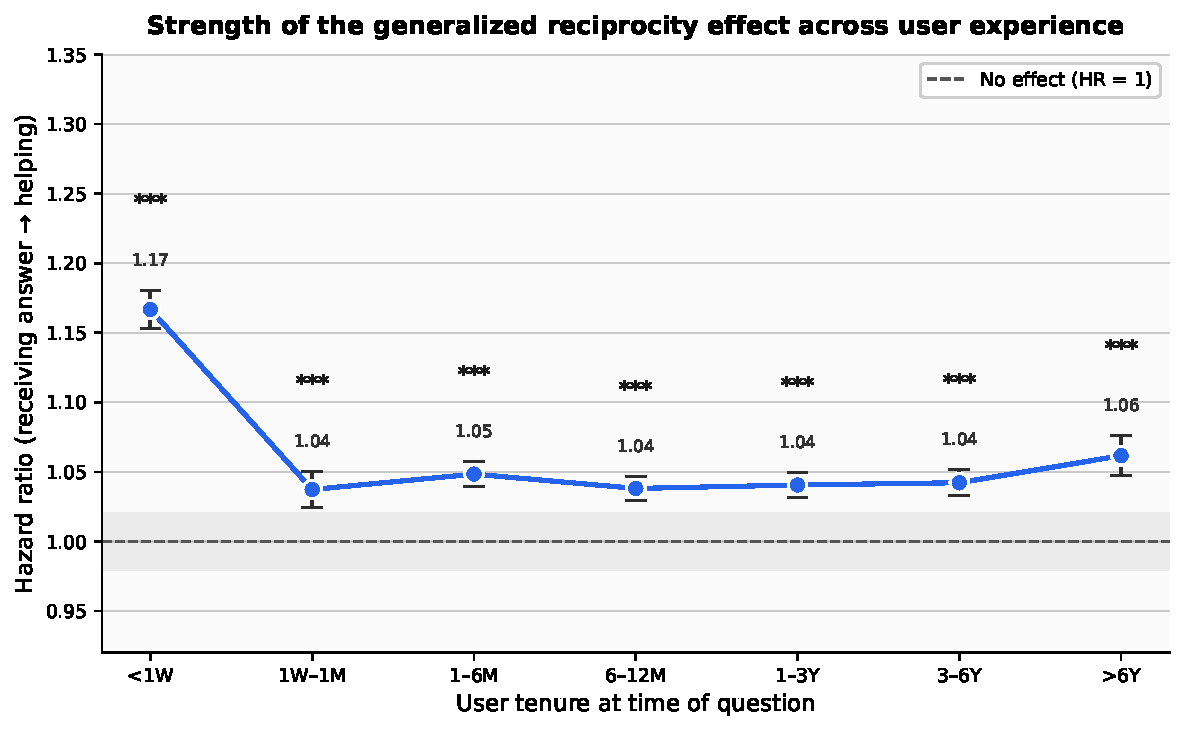
\includegraphics[width=\textwidth]{analysis/output_figures/strength_rec.pdf}
\caption{Strength of the generalized reciprocity effect across user experience. Bars show the hazard ratio for the treatment effect by tenure bucket. Error bars indicate 95\% confidence intervals.}
\label{fig:strength_rec}
\end{figure}

\begin{landscape}
\begin{table}
\caption{Cox Regression Results: Effect of Receiving an Answer on Helping Hazard}
\label{tab:main_results}
\centering
\scriptsize
\setlength{\tabcolsep}{1.5pt}
\resizebox{\linewidth}{!}{%
\begin{tabular}{@{}>{\raggedright\arraybackslash}p{2.55cm}*{7}{c}@{}}
\toprule
 & \shortstack[c]{$<$ 1\\Week} & \shortstack[c]{1 Wk--\\1 Mo} & \shortstack[c]{1--6\\Mo} & \shortstack[c]{6--12\\Mo} & \shortstack[c]{1--3\\Yr} & \shortstack[c]{3--6\\Yr} & \shortstack[c]{$>$ 6\\Yrs} \\
\midrule
\multicolumn{8}{@{}l}{\textit{Treatment Effect (DiD): post-answer vs.\ pre-question}} \\
\hspace{1em}Received Answer (net post-answer) & 0.1021*** & -0.0302*** & -0.0134** & -0.0055 & -0.0057 & -0.0317*** & -0.0050 \\
 & (0.0067) & (0.0085) & (0.0049) & (0.0055) & (0.0048) & (0.0062) & (0.0109) \\
\hspace{1em}\textit{Hazard Ratio [95\% CI]} & [1.09, 1.12] & [0.95, 0.99] & [0.98, 1.00] & [0.98, 1.01] & [0.98, 1.00] & [0.96, 0.98] & [0.97, 1.02] \\[4pt]
\multicolumn{8}{@{}l}{\textit{\quad Decomposition (nested time-varying terms)}} \\
\hspace{2em}Waiting period ($\times$ Post-Question) & 0.0410*** & -0.0420*** & -0.0482*** & -0.0177* & -0.0165** & -0.0131\textdagger & -0.0013 \\
\hspace{2em}Answer arrival ($\times$ Post-Answer Received) & 0.0611*** & 0.0119 & 0.0348*** & 0.0122\textdagger & 0.0108\textdagger & -0.0186** & -0.0037 \\[4pt]
\midrule
N & 2,667,533 & 1,054,458 & 2,788,155 & 2,055,064 & 4,312,164 & 2,311,821 & 1,063,329 \\
Events & 288,974 & 231,097 & 732,719 & 601,239 & 840,925 & 540,767 & 177,398 \\
\bottomrule
\multicolumn{8}{@{}l}{\footnotesize N = unique questions (treated + control) in the Cox sample. Within each column, treated vs.\ control counts can differ because tenure is defined per question.} \\
\multicolumn{8}{@{}l}{\footnotesize Cox-table standard errors are model-based; matched-pair bootstrap uncertainty is reported separately when generated.} \\
\multicolumn{8}{@{}l}{\footnotesize $^{***}p<0.001$; $^{**}p<0.01$; $^{*}p<0.05$; $^{\dagger}p<0.1$} \\
\end{tabular}%
}
\end{table}
\end{landscape}




%----------------------------------------------------------------------
\subsection{Response Time Moderation (H3)}
%----------------------------------------------------------------------

Hypothesis~3 predicted that faster responses would strengthen the reciprocity effect. Table~\ref{tab:speed_results} reports the interaction between the treatment effect and log response time, estimated separately by tenure bucket. In the revision data, the speed interactions are positive across all tenure groups ($\gamma$\,$\approx$\,0.05--0.33, all $p < .001$), indicating that longer response times are associated with a more negative post-answer treatment coefficient in the speed-augmented specification. For example, newcomers show $\gamma = 0.0497$ (SE\,=\,0.0020), users with one to six months show $\gamma = 0.0894$ (SE\,=\,0.0015), and users with more than six years show $\gamma = 0.3274$ (SE\,=\,0.0027).

To test Hypothesis~3, we examine how the treatment effect varies with answer speed, both continuously (Table~\ref{tab:speed_results}) and across discrete response-time bins (Table~\ref{tab:response_time_bins}, Figure~\ref{fig:interaction_effect}). The response-time moderation of the treatment effect is the sum $\gamma + \delta$, just as the base effect is $\beta_2 + \beta_4$. This net moderation is small and changes sign across the tenure range --- modestly positive among newcomers and modestly negative among veterans --- rather than uniformly favoring fast answers. The discrete-bin estimates, read as the summed post- versus pre-question contrast within each bin, likewise do not reproduce the clean monotone pattern reported for the earlier sample; the sharp bin-to-bin swings visible when only the answer-arrival increment is plotted are an artifact of the waiting period entering the model at longer response times, not a behavioral discontinuity. Taken together, the evidence for Hypothesis~3 is mixed: answer speed moderates the effect weakly and inconsistently, and we treat the response-time results as exploratory. % TODO(re-run): refresh net moderation (gamma+delta) and per-bin summed HRs from regenerated Tables~\ref{tab:speed_results} and \ref{tab:response_time_bins}.

\begin{landscape}
\begin{table}[H]
\caption{Response Time Moderation of the Reciprocity Effect}
\label{tab:speed_results}
\centering
\footnotesize
\begin{tabular}{@{}lccccccc@{}}
\toprule
 & < 1 Week & 1 Week - 1 Month & 1 - 6 Months & 6 - 12 Months & 1 - 3 Years & 3 - 6 Years & > 6 Years \\
\midrule
\multicolumn{8}{@{}l}{\textit{Base Treatment Effect}} \\
\hspace{1em}Received Answer $\times$ Post-Answer Received & 0.0855*** & 0.0968*** & 0.1007*** & 0.0925*** & 0.0698*** & 0.0476*** & 0.0337** \\
 & (0.0130) & (0.0133) & (0.0126) & (0.0126) & (0.0125) & (0.0126) & (0.0128) \\[4pt]
\multicolumn{8}{@{}l}{\textit{Response Time Interaction}} \\
\hspace{1em}Treatment $\times$ log(Response Time) & 0.0125* & -0.0101* & -0.0097* & -0.0038 & 0.0074\textdagger & 0.0256*** & 0.0241*** \\
 & (0.0053) & (0.0048) & (0.0044) & (0.0043) & (0.0044) & (0.0047) & (0.0051) \\[4pt]
\multicolumn{8}{@{}l}{\textit{Waiting Period $\times$ Response Time}} \\
\hspace{1em}Post-Question $\times$ log(Response Time) & -0.0118* & -0.0181*** & -0.0132** & -0.0087\textdagger & 0.0104* & 0.0197*** & 0.0143** \\[4pt]
\midrule
Intervals & 1,999,916 & 1,839,458 & 1,999,744 & 2,000,131 & 2,000,142 & 1,999,282 & 2,000,046 \\
Events & 30,606 & 63,928 & 79,080 & 86,418 & 80,654 & 60,295 & 41,276 \\
\bottomrule
\multicolumn{8}{@{}l}{\footnotesize $^{***}p<0.001$; $^{**}p<0.01$; $^{*}p<0.05$; $^{\dagger}p<0.1$} \\
\end{tabular}
\end{table}
\end{landscape}



\begin{figure}[h]
\centering
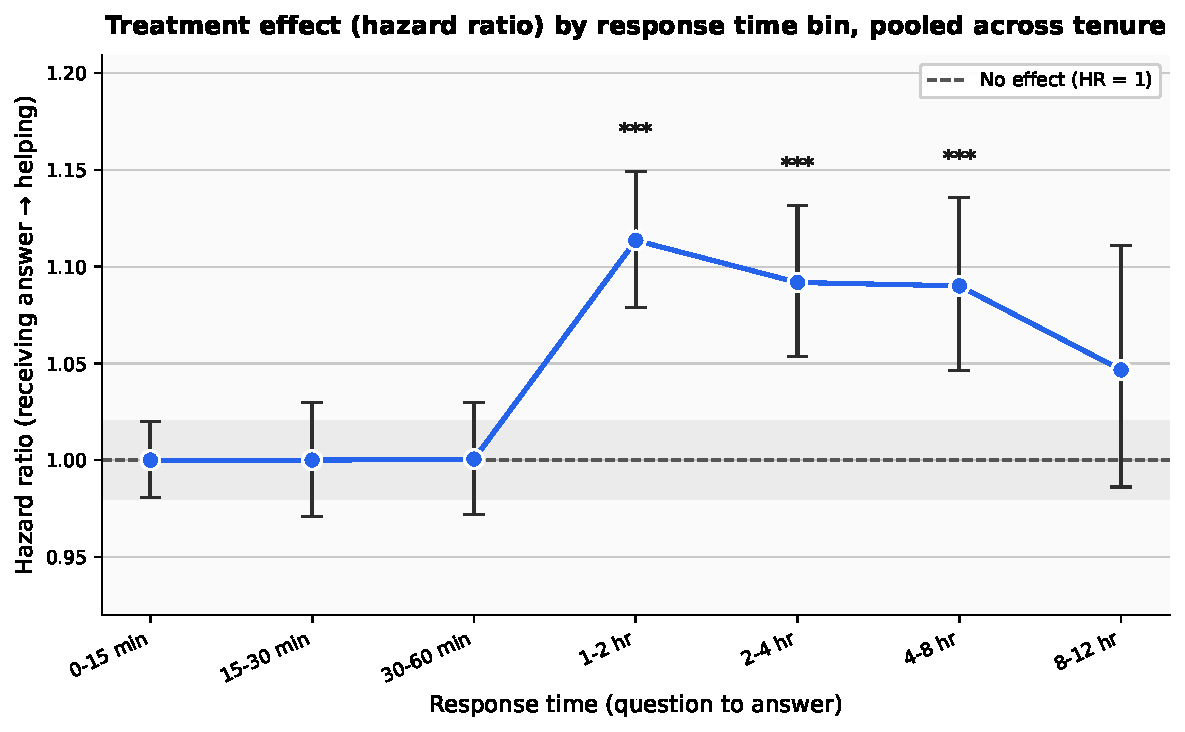
\includegraphics[width=\textwidth]{analysis/output_figures/interaction_effect.pdf}
\caption{Treatment effect (hazard ratio) by response time bin, pooled across all tenure buckets. Each point represents the estimated hazard ratio of the treatment indicator within that response-time bin, relative to the matched control. Error bars indicate 95\% confidence intervals.}
\label{fig:interaction_effect}
\end{figure}

\begin{table}[H]
\caption{Treatment Effect by Response-Time Bin}
\label{tab:response_time_bins}
\centering
\footnotesize
\begin{tabular}{@{}lrrrr@{}}
\toprule
\textbf{Response time} & \textbf{HR} & \textbf{95\% CI} & \textbf{N} & \textbf{Events} \\
\midrule
0-15 min & 0.99 & [0.97, 1.01] & 17,412,740 & 3,598,284 \\
15-30 min & 0.99 & [0.96, 1.02] & 13,934,456 & 2,655,887 \\
30-60 min & 1.22*** & [1.19, 1.25] & 13,549,736 & 2,559,608 \\
1-2 hr & 1.03* & [1.00, 1.06] & 13,211,144 & 2,491,230 \\
2-4 hr & 1.03 & [0.99, 1.06] & 12,958,927 & 2,439,543 \\
4-8 hr & 1.00 & [0.97, 1.03] & 12,762,008 & 2,403,607 \\
8-12 hr & 0.97 & [0.93, 1.01] & 12,464,162 & 2,346,654 \\
12-24 hr & 1.04* & [1.00, 1.07] & 12,645,932 & 2,384,160 \\
1-3 days & 1.04** & [1.01, 1.08] & 12,592,667 & 2,400,019 \\
$>$3 days & 1.01 & [0.98, 1.05] & 12,391,574 & 2,390,995 \\
\bottomrule
\multicolumn{5}{@{}l}{\footnotesize Cox-table standard errors are model-based; matched-pair bootstrap 95\% CIs for the pooled DiD are in Table~\ref{tab:pair_bootstrap}.} \\
\multicolumn{5}{@{}l}{\footnotesize Events = helping events in the full analysis sample (after time rounding); when interval rows exceed the fit cap, estimation uses a matched-pair subsample but Events still refer to the full sample.} \\
\multicolumn{5}{@{}l}{\footnotesize Each row fits Model A to treated questions in that response-time bin plus the full no-answer control pool.} \\
\multicolumn{5}{@{}l}{\footnotesize HR is the answer-arrival increment ($\beta_4$, is\_treated\_active) at answer arrival; the summed DiD contrast is reported in the pooled regression tables.} \\
\multicolumn{5}{@{}l}{\footnotesize $^{***}p<0.001$; $^{**}p<0.01$; $^{*}p<0.05$; $^{\dagger}p<0.1$} \\
\end{tabular}
\end{table}

One reading of the anticipatory-engagement pattern draws on platform session dynamics. When a user posts a question, they enter a state of active, engaged waiting --- remaining on the platform and browsing other questions during the interval before their answer arrives --- which would elevate their helping during the waiting period regardless of whether an answer ever comes. On this account the negative answer-arrival increment reflects the resolution of that pending state: once the answer lands, the reason to stay engaged is discharged, and helping subsides toward baseline. This interpretation is speculative. It is consistent with the large waiting-period term and the negative arrival increment, but our data cannot distinguish it from a simpler selection account in which users whose questions attract answers were more active to begin with, and we do not observe the session boundaries (logins, logouts, inactivity gaps) that a direct test would require. % AUTHOR DECISION: the earlier "re-engagement window / inverted-U" contribution is not supported once the nested terms are summed; consider demoting it from a headline contribution to an exploratory conjecture, or cutting it.

Figure~\ref{fig:help_rate_adoption_pooled} provides descriptive support. The plot compares users who have received an answer (red) and users who will receive one but are still waiting (blue). The gap between users who received help and those who still wait is small initially, then widens and converges at later responses, consistent with re-engagement being most likely in the intermediate response-time range. Tenure-stratified versions of this figure are in Appendix Figure~\ref{fig:help_rate_adoption_by_tenure}.

\begin{figure}
\centering
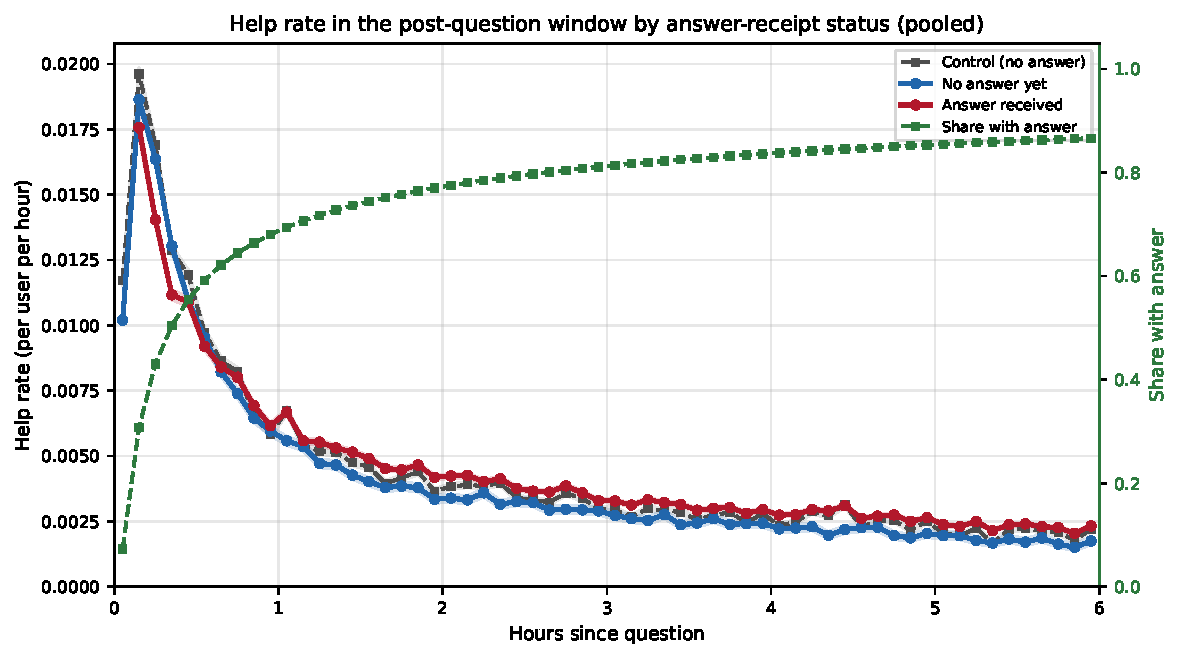
\includegraphics[width=\textwidth]{analysis/output_figures/help_rate_adoption_pooled.pdf}
\caption{Help rate in the post-question window by answer-receipt status, pooled across all tenure buckets. Grey dashed: matched control users who received no answer. Blue: treated users who have not yet received an answer (No answer yet). Red: treated users who have already received an answer (Answer received). Green dashed (right axis): cumulative share of treated users who have received an answer by each hour.}
\label{fig:help_rate_adoption_pooled}
\end{figure}

%======================================================================
\section{Discussion}
\label{sec:discussion}
%======================================================================

%----------------------------------------------------------------------
\subsection{Methodological Contribution}
%----------------------------------------------------------------------

A persistent difficulty in studying generalized reciprocity from platform data is that the same user characteristics that predict seeking help also predict giving it. Active, engaged users are more likely both to post questions and to post answers, so correlations between help received and help given can reflect differences in user engagement rather than any causal response to receiving help. Prior observational studies that report positive associations between help-seeking and subsequent helping behavior without accounting for this selection \citep{baker_paying_2014, chen_engaging_2018, joyce_predicting_2006} may have overstated the role of reciprocity. The matched DiD survival design developed here addresses this confound by comparing changes in helping behavior, before and after question posting, between users whose questions received answers and propensity-score-matched users whose questions did not. The waiting-period covariate makes any pre-answer divergence between treated and control users visible, so that such a divergence is measured rather than silently absorbed into the treatment effect --- a diagnostic that, in the present data, turns out to matter (see the anticipatory-engagement pattern in the Results). Together, these features provide a more credible basis for causal inference than prior designs, and the estimated post-answer elevation is substantially smaller than many earlier reports, consistent with the view that prior estimates were partially confounded by baseline activity.

%----------------------------------------------------------------------
\subsection{Reciprocity as a Contributor-Recruitment Mechanism}
%----------------------------------------------------------------------

The theoretical account developed in this paper treats generalized reciprocity not as a uniform driver of community cooperation, but as a mechanism whose salience varies with a user's position on the trajectory from newcomer to established contributor. The summed treatment effect is consistent with this account: it is largest among the newest users and declines to near zero among the most experienced. Two features counsel caution, however, before reading the gradient as evidence that reciprocity recruits newcomers. First, the gradient resides almost entirely in \textit{anticipatory engagement} --- the pre-answer activity of users whose questions are about to be answered --- rather than in the response to the answer itself, which is roughly flat across tenure. Second, because anticipatory engagement precedes treatment, part of what appears as stronger newcomer reciprocity may instead be stronger newcomer selection into being answered. The contributor-recruitment interpretation is thus plausible but not established; the cleanest test would isolate cases in which the waiting period is negligible, so that anticipatory engagement cannot contribute to the estimated effect.

If this gradient does reflect reciprocity rather than anticipatory engagement, it has implications for how reciprocity's role in online communities should be understood. If the effect were uniform across experience levels, reciprocity could plausibly be treated as a general engine of cooperative behavior, sustaining helping throughout a community's membership. The observed attenuation would instead suggest a narrower role: reciprocity is most operative at the point of entry, providing an early push into helping before community-specific motivations are established. Newcomers lack the experience to value platform-specific incentives such as reputation accumulation or norm identification. The general moral impulse to reciprocate, what \citet{levine_logic_2020} terms the logic of universalization, is more prominent precisely because these community-specific motivations have not yet taken hold.

As users accumulate experience, this account predicts that community-specific incentives gradually displace the general reciprocal impulse. This is consistent with theories of norm displacement \citep{benabou_incentives_2006}, which show how the introduction of external incentives can crowd out moral motives. On Stack Overflow, reputation systems and status markers provide salient, community-specific reasons to help that are not available to newcomers. The absence of a detectable reciprocity effect among the most established users is consistent with this displacement account, though we cannot directly observe the motivational shift that the theory posits.

This reframing also helps account for the inconsistency of findings in the prior literature. Studies that draw primarily on samples of experienced users, or that aggregate across experience levels dominated by experienced contributors, should find weaker reciprocity effects under this account. Studies that capture behavior early in the user trajectory should find stronger ones. The variation in prior findings may thus reflect not noise or methodological failure, but genuine 
heterogeneity in the effect across the user population.

%----------------------------------------------------------------------
\subsection{Platform Session Dynamics and the Re-engagement Window}
%----------------------------------------------------------------------

The response-time analysis was intended to test the prediction, derived from laboratory studies of gratitude, that faster help produces stronger reciprocity. Once the two response-time interactions are combined into the net moderation of the treatment effect ($\gamma + \delta$), that moderation is small and inconsistent in sign across tenure, and the discrete-bin pattern does not reproduce the monotone relationship such theories predict. We therefore find little support for a strong version of the immediacy hypothesis in this field setting, and we treat the response-time results as exploratory.

To the extent that response time matters at all, the pattern is more consistent with platform session dynamics than with graded emotional immediacy. An answer that arrives while a user is still actively waiting may simply discharge the engagement that the act of asking created, rather than triggering a reciprocal impulse whose intensity scales with speed; on this reading the elevated waiting-period helping is a feature of the session, not a response to the answer. We advance this only as a conjecture. Our data cannot distinguish it from a simpler selection account --- users whose questions attract answers are more active to begin with --- because we do not observe the session boundaries (logins, logouts, inactivity gaps) that a direct test would require. % AUTHOR DECISION: the earlier "re-engagement window / inverted-U" claim is not supported once the nested terms are summed. Consider demoting this subsection from a headline contribution to a brief exploratory note, or cutting it.

The response-time results bear only weakly on the norm-displacement account. The summed treatment effect is near zero among the most experienced users, and the response-time moderation is likewise negligible for that group, which is at least consistent with the mechanism as a whole having faded rather than merely dampened. Given how weak and inconsistent the response-time moderation is across tenure, however, we do not lean on this pattern as evidence for displacement.

%----------------------------------------------------------------------
\subsection{Implications for Platform Design}
%----------------------------------------------------------------------

Because the reciprocity effect is concentrated among newcomers, the practical leverage that platforms can derive from it lies primarily in contributor recruitment rather than in sustaining contributions from established members.

The most direct implication is that platforms seeking to grow their contributor base should prioritize ensuring that new users receive answers to their questions. Answer receipt itself, rather than its speed, is the more important factor: the base effect is present across a wide range of response times, while speed moderation is secondary. Recommendation systems and visibility-boosting mechanisms that surface questions from new users to experienced answerers are, under this account, doing double work: they improve new users' direct experience and increase the probability that those users convert into contributors.

Our results do not support a distinct response-time lever for design. The earlier suggestion that intermediate response times are uniquely effective does not survive the corrected specification, in which the net response-time moderation is small and inconsistent, so we do not recommend timing interventions built on it. The practical emphasis returns to answer receipt itself: ensuring that newcomers' questions are answered at all, and that answer notifications are salient, is better supported than any intervention keyed to a particular response-time window.

A further implication concerns the increasing prevalence of AI-generated answers on question-and-answer platforms. If AI assistance substitutes for human responses, the human-to-human interaction that creates the moral and emotional basis for generalized reciprocity may decline. Given that the effect is concentrated among newcomers, this substitution could impair the contributor-recruitment function that reciprocity appears to serve, reducing the pipeline of new contributors who currently receive an early push into helping from the experience of being helped by a human community member.

%----------------------------------------------------------------------
\subsection{Limitations}
%----------------------------------------------------------------------

Several limitations constrain the conclusions that can be drawn from this analysis.

The most important is a departure from the design's parallel-trends assumption. Treated and control users diverge during the waiting period, before any answer arrives, and this anticipatory engagement is large --- comparable in magnitude to the post-answer effect itself. Our design makes this pre-trend visible rather than assuming it away, but it cannot fully remove it: propensity-score matching balances pre-question characteristics, yet whether a question is ultimately answered is correlated with the asker's contemporaneous platform activity, which matching on pre-question covariates does not capture. As a result, the summed treatment effect is best read as an upper bound on reciprocity, and the answer-arrival component alone --- which nets out the pre-trend --- is negative rather than positive. We cannot cleanly separate a reciprocal response to receiving help from selection into being answered, and the tenure gradient in the effect is, correspondingly, largely a gradient in anticipatory engagement rather than in the response to the answer. Stronger identification would require an instrument for answer receipt, or a design restricted to near-instantaneous answers in which the waiting period, and hence anticipatory engagement, is negligible.

Beyond identification, the design captures a behavioral response but cannot identify the psychological mechanism producing it. Gratitude, moral obligation, and the re-engagement dynamics of platform sessions are all consistent with the observed patterns, and the data do not allow us to distinguish among them. Future work combining behavioral records with experience-sampling measures of emotional state or moral reasoning during platform use could help disentangle these pathways.

The identification strategy rests on the assumption that, conditional on the matched covariates and the DiD structure, answer receipt is approximately independent of the potential outcomes for helping behavior. The propensity score matching substantially improves the comparability of treated and control observations, as confirmed by post-matching balance diagnostics. Unobserved time-varying factors, including changes in workload, access to alternative information sources, or exogenous variation in a user's availability, could nonetheless bias the estimates in ways that the design cannot rule out.

Response time may partially proxy for question characteristics not fully captured by the tag-level answer rate, since questions that attract fast responses may differ systematically from those that wait. Future work with random treatment or finer-grained measures of question difficulty, such as text-based complexity or specificity scores, could provide a cleaner test of the response time mechanism.

The re-engagement window interpretation rests on indirect evidence: the non-linearity in the discrete-bin analysis, the broadly negative continuous speed interactions, and descriptive patterns in the help-rate figures. Direct tests would require session-level data, including login and logout timestamps or inactivity-based session boundaries, to confirm that the peak effect occurs among users who left and were drawn back by the answer notification, and that very fast answers disproportionately end active sessions. This remains an important direction for future work.

Stack Overflow is a large, relatively anonymous platform built around technical question-answering. The mechanisms identified here are likely to operate in other knowledge-sharing communities, but the specific patterns, including the tenure gradient, the shape of the re-engagement window, and the attenuation at high experience levels, may differ in smaller or more intimate settings, in intra-organizational platforms where social ties moderate motivation, or on platforms with different incentive structures.

Finally, the analysis establishes that reciprocity declines with experience but does not characterize what replaces it. The theoretical argument implicates com\-munity-spe\-cific norms and status motives, but testing this account would require integrating behavioral analysis with direct measures of those alternative mechanisms, for instance, through surveys or experimental manipulations of reputation visibility.

%=============================================================
\section{Conclusion} \label{sec:conclusion} %=============================================================
Generalized reciprocity is widely theorized as a mechanism sustaining cooperation on knowledge-sharing platforms, but observational evidence is limited by a persistent confound: active users are more likely both to seek help and to give it, regardless of whether their questions are resolved. Our matched difference-in-differences survival design confronts this confound directly, and the result is a more measured picture than the literature's. Users who receive an answer do help others at a modestly higher rate afterward (pooled HR\,$\approx$\,1.16), and that elevation is largest among newcomers and negligible among veterans. But the design also reveals what a cleaner-looking estimate would have hidden: most of the treated--control gap opens while users await an answer, before any help has been received. This anticipatory engagement, not the answer itself, carries the tenure gradient, and it marks the boundary of what observational data can settle here. Receiving help may well nudge newcomers toward helping others; our estimates are consistent with that story but cannot, on their own, separate it from the simpler fact that users whose questions get answered were more engaged to begin with. Distinguishing the two is the task we leave to designs with exogenous variation in whether, and how quickly, help arrives.